\documentclass[a4paper,11pt,dvipdfmx]{jsarticle}

\usepackage{bm}
\usepackage[dvipdfmx]{graphicx}
\usepackage[subrefformat=parens]{subcaption}
\usepackage[dvipdfmx]{color}
\usepackage{ascmac}
\usepackage{siunitx}
\usepackage{otf}
\pagestyle{plain}
\usepackage{float}
\usepackage[dvipdfmx]{hyperref}
\usepackage{pxjahyper}
\usepackage{here}
\usepackage{titlesec}
\titleformat*{\section}{\LARGE\bfseries}
\titleformat*{\subsection}{\normalsize\bfseries}
\usepackage{url}
\usepackage{comment}
\usepackage[table,xcdraw]{xcolor}
\hypersetup{% hyperrefオプションリスト
setpagesize=false,
 bookmarksnumbered=true,%
 bookmarksopen=true,%
 colorlinks=true,%
 linkcolor=blue,
 citecolor=blue,
}

\begin{document}


\subsection{ターゲット}
1.6節より陽子ビームを当てるターゲットにポリエチレンと金を利用する。ポリエチレンにはコープキッチン用ポリ袋を、金にはカタニ産業の金箔24Kを利用する。

\subsubsection{ターゲットの厚さ}
各社の出すターゲットの厚さの精度が低いため、ポリエチレンはµメーターで計測し、金は密度と体積が分かった状態で質量を計測し厚さを求めた。それぞれの表記値と計測値を表\ref{thickness}に示す。

\begin{table}[H]
 \centering
 \begin{tabular}{cccll}
 \cline{1-3}
  \multicolumn{1}{|c|}{}       & \multicolumn{1}{c|}{表記値}    & \multicolumn{1}{c|}{計測値}           &  &  \\ \cline{1-3}
  \multicolumn{1}{|c|}{ポリエチレン} & \multicolumn{1}{c|}{10µm}   & \multicolumn{1}{c|}{11.5±0.2µm}    &  &  \\ \cline{1-3}
  \multicolumn{1}{|c|}{金}      & \multicolumn{1}{c|}{約0.1µm} & \multicolumn{1}{c|}{0.161±0.006µm} &  &  \\ \cline{1-3}
  \multicolumn{1}{l}{}         & \multicolumn{1}{l}{}        & \multicolumn{1}{l}{}               &  & 
 \end{tabular}
 \caption{ターゲットの厚さの表記値と計測値}
 \label{thickness}
\end{table}

\subsubsection{ターゲットホルダー}
ポリエチレンはセロハンテープでアルミ板に張り付け、ターゲットに水平方向から検出器の角度が小さい場合にも測定できるように固定した。金に関しては非常に薄くセロハンテープ等で固定することは不可能であるため、先行研究と同様に2枚のアルミ板でターゲットを挟み、ネジで固定した。このターゲットホルダーはターゲットが露出す津中心部が削られているため、なるべく大きな散乱角に対応することが可能である。図\ref{poli}にポリエチレンのターゲットを、図\ref{gold}に金のターゲットを、図\ref{goldtokutyou}に金のターゲットホルダーの特徴を示す。
\par
ターゲットをポリエチレンにして強いビームを一定時間当てると焦げが出来る、この焦げに合わせてターゲットとビームストッパーの位置調整を行った。焦げが出来たポリエチレンのターゲットを図\ref{koge}に示す。

  \begin{figure}[H]
    \centering
    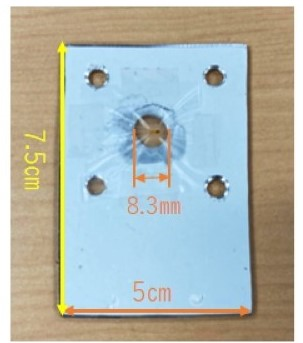
\includegraphics[width=35mm]{picture/setup/poli.jpg}
    \caption{ポリエチレンのターゲット}
    \label{poli}
  \end{figure}
  
  \begin{figure}[H]
    \begin{minipage}{0.5\hsize}
     \begin{center}
      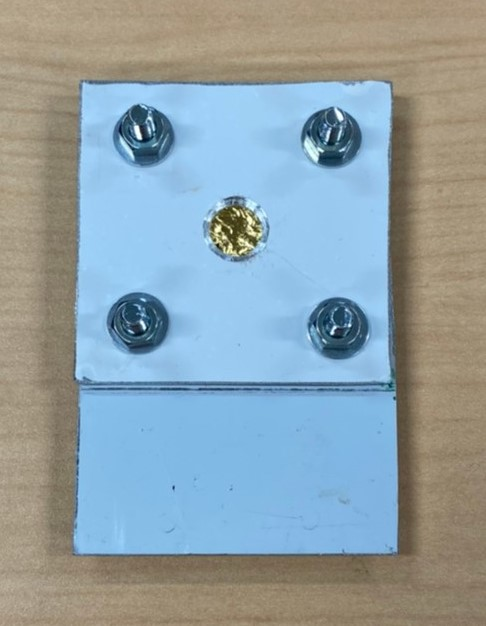
\includegraphics[width=30mm]{picture/setup/gold.jpg}
     \end{center}
     \caption{金のターゲット}
     \label{gold}
    \end{minipage}
    \begin{minipage}{0.5\hsize}
     \begin{center}
      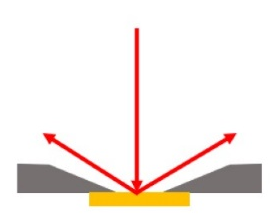
\includegraphics[width=40mm]{picture/setup/goldtokutyou.png}
     \end{center}
     \caption{金のターゲットホルダーの特徴}
     \label{goldtokutyou}
    \end{minipage}
  \end{figure}
  
  \begin{figure}[H]
    \centering
    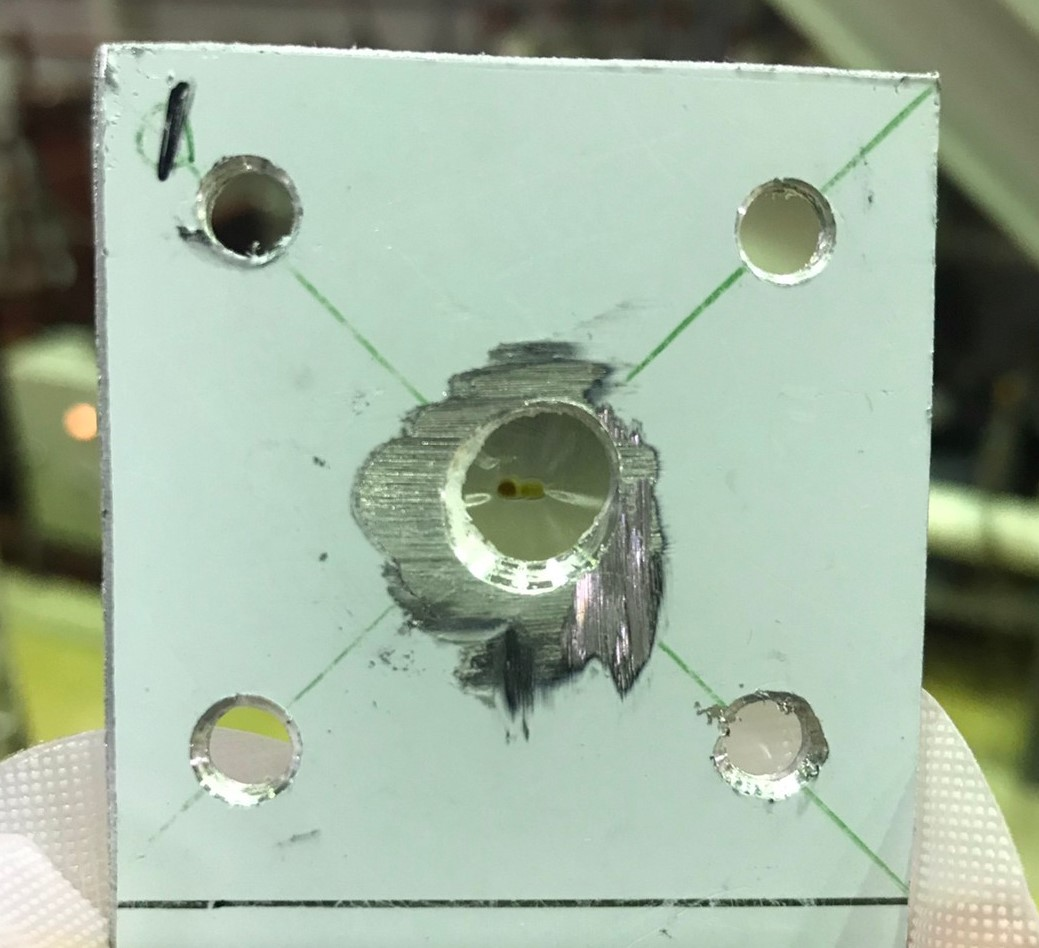
\includegraphics[width=35mm]{picture/setup/koge.jpg}
    \caption{焦げができたポリエチレンのターゲット}
    \label{koge}
  \end{figure}

\subsection{まとめ}
精度の良いピークを得るために、ビームストッパーを設置しバックグラウンドを防ぐこと、ターゲット(ポリエチレン)を直接アルミ板に貼り付け、ターゲットに水平方向から検出器の角度が小さい場合も測定できるようにしたこと。ポリエチレンにできたビームによるこげからビームストッパーの位置を決定することをした。また、散乱粒子と反跳粒子の両方を観測するため、検出回路をもう1台制作した。さらにターゲットの厚さを自ら計測することで精度の良い実験を行う工夫をした。

\end{document}